%----------------------------------------------------------------------------
\chapter{Background}
%----------------------------------------------------------------------------

This chapter provides some theoretical background of the contributions presented in this thesis. First of all, the necessary basics of formal language and automaton theory are introduced, afterwards we discuss automaton learning algorithms.

\section{Basics of automaton theory}

First, we introduce the fundamentals of formal language theory, which are essential in order to understand automaton theory. Atomic elements of formal languages are alphabets, characters and words.

\begin{definition}[Alphabet]
	Let $\Sigma$ be a finite, non-empty set. $\Sigma$ is an Alphabet, its elements are symbols or characters.
\end{definition}

\begin{definition}[Word]
	If $\Sigma$ is an alphabet, then any finite sequence comprised of the symbols of $\Sigma$ are words (or Strings). $\Sigma^{n}$ represents the set of every n length word in $\Sigma$. The set of every word under an alphabet, formally $\bigcup\limits_{n>0}^{} \Sigma^{n}$ is denoted by $\Sigma^{*}$. The empty word is denoted by $\epsilon$.
\end{definition}

Words can be constructed using other words, the following definition defines these relations.

\begin{definition}[Prefixes, Substrings and Suffixes]
	If $w = uvs$, where $w, u, v, s\in\Sigma^*$, $u$ is the prefix, $v$ is the substring, and $s$ is the suffix of $w$.
\end{definition}

Using these atomic elements of formal language theory, the definition of formal language theory can be seen as follows.

\begin{definition}[Formal Language]
	An arbitrary set of words under an Alphabet $\Sigma$ is a Language. Formally: $L\subseteq\Sigma^{*}$.
\end{definition}

\begin{definition}[Prefix-closure]
	Let $L\subseteq\Sigma^*$ and $L' = \{u\in\Sigma^*, v\in\Sigma^* : uv\in L\}$. In other words, L' is the set containing all the prefixes of every word of L. L is prefix-closed if $L = L'$.
\end{definition}

We will expand on formal languages more once we have a basic understanding of automatons. 

Informally, Automatons, or automata are mathematical constructs which are able to determine if a sequence of inputs should be accepted or rejected. A bit more precisely, automata consist of states and is always in one of them. Starting from an initial state, based on the inputs received, the automaton changes, "moves" between states. Essentially, for every one of the inputs, based on the current state the automaton is in, it determines whether to keep, or change its current state. In order to determine if an input sequence should be accepted or not, some states are special, accepting states. If after processing a sequence of inputs, the final state of the automaton is accepting, the input sequence is accepted. If not, the input is rejected.


One of the most simple automaton is the Deterministic Finite Automaton.

\begin{definition}[Deterministic Finite Automaton]
	A Deterministic Finite Automaton is a Tuple of $ DFA=(S,s_{0},\Sigma,\delta,F) $, where: 
	\begin{itemize}
		\item S is a finite, non-epty set containing the states of the automaton,
		\item $s_{0} \in S$ is the initial state,
		\item $\Sigma$ is a finite Alphabet,
		\item $\delta: S\times \Sigma \to S$ is a transition function,
		\item $F\subseteq S$ is a set of the accepting states of the automaton. 
	\end{itemize}
\end{definition}


An example of a DFA (Deterministic Finite Automaton) from\cite{Steffen2011} can be seen in Example \ref{ex:dfaexample}.

\begin{example}
	\label{ex:dfaexample}
	See Fig. \ref{fig:dfaexample}. This example has four states, $S = \{q_0, q_1, q_2, q_3\}$ (hence $|S| = 4$). The initial state is marked by the start arrow, so $s_0 = q_0$. The alphabet can be inferred as $\Sigma = \{a, b\}$ because of the deterministic in Deterministic Finite Automaton, meaning every state must deterministically know what input causes what action. This means, that every state must have every member of the alphabet listed in its transitions. Transitions are visualized as $q_0$ $\xrightarrow[]{\text{a}}$ $q_1$ given by the transition function (in this example) $\delta(q_0, a) = q_1$. The whole of the transition function in a table form can be seen in Table \ref{tab:dfaexampledelta}. Finally, the accepting states, or in this case, accepting state of the automaton is $F = \{q_3\}$.
\end{example}
 

When talking about automata, it is important to discuss runs. A run of an automaton is to test for a certain input (word), if it is accepted or rejected. See Example \ref{ex:dfaruns}.

\begin{example}
	\label{ex:dfaruns}
	A run of Fig. \ref{fig:dfaexample} with an input of $\{a, a, a\}$ would (following the transition function) end in state $q_3$ meaning the input is accepted. A rejected input could be $\{a, b, b\}$, which would stop at state $q_1$, a non-accepting state. On deeper examination, one can see, that this automaton only accepts runs with inputs containing $4i+3 a$.
\end{example}

\begin{figure}[H]
	\centering
	\begin{tikzpicture}[shorten >=1pt,node distance=3cm,on grid,auto] 
	\node[state,initial] (q_0)   {$q_0$}; 
	\node[state] (q_1) [right=of q_0] {$q_1$}; 
	\node[state] (q_2) [below=of q_0] {$q_2$}; 
	\node[state,accepting](q_3) [right=of q_2] {$q_3$};
	\path[->] 
	(q_0) edge  node {a} (q_1)
	edge [loop below] node {b} ()
	(q_1) edge  node  {a} (q_2)
	edge [loop below] node {b} ()
	(q_2) edge  node [swap] {a} (q_3) 
	edge [loop above] node {b} ()
	(q_3) edge  node [swap] {a} (q_0)
	 edge [loop above] node {b} () ;
	\end{tikzpicture}
	\caption{A simple DFA}
	\label{fig:dfaexample}
\end{figure}

\begin{table}[H]
\centering
\begin{tabular}{|c|cccc|}
	\hline
	$\delta$ & $q_0$ & $q_1$ & $q_2$ & $q_3$\\ \cline{1-5}
	a & $q_1$ & $q_2$ & $q_3$ & $q_0$ \\	
	b & $q_0$ & $q_1$ & $q_2$ & $q_3$ \\	\hline
\end{tabular}
\caption{The transition function of the automaton seen in Fig. \ref{fig:dfaexample}}
\label{tab:dfaexampledelta}
\end{table}

DFAs are great to model system behavior based on inputs, but in order to work with reactive systems, we also need to handle outputs. Mealy machines are automata designed to do just this, while becoming more complicated with regard to accepting inputs.


\begin{definition}[Mealy machine]
	A Mealy machine or Mealy automaton is a Tuple of $ M=(S,s_{0},\Sigma,\Omega,\delta,\lambda) $, where:
	\begin{itemize}
		\item S is a finite, non-empty set containing the states of the automaton,
		\item $s_{0} \in S$ is the initial state,
		\item $\Sigma$ is the input alphabet of the automaton,
		\item $\Omega$ is the output alphabet of the automaton,
		\item $\delta: Q\times \Sigma \to Q$ is the transition function and
		\item $\lambda: Q\times \Sigma \to \Omega$ is the output function. 
	\end{itemize}
\end{definition}

Mealy machines can be regarded as deterministic finite automata over the union of the input alphabet and an output alphabet with just one rejection state, which is a sink, or more elegantly, with a partially defined transition relation. 

An example of a deterministic Mealy machine can be seen in Example \ref{ex:coffeemealy}.

\begin{example}
	\label{ex:coffeemealy}
	An example of a deterministic Mealy machine can be seen in Fig. \ref{fig:coffeemealy}. The formal definition of the automaton can be seen below.
	\begin{itemize} 
		\item $S = \{a, b, c, d, d', e, f\}$ 
		\item $s_0 = a$
		\item $\Sigma = \{water, pod, button, clean\}$
		\item $\Omega$ = \{$\checkmark$, \Coffeecup, $\star$\}
	\end{itemize}
	The transitions, as seen in Fig. \ref{fig:coffeemealy} are visualized as $s_0$ $\xrightarrow[]{\text{input/output}}$ $s_1$, which denotes the machine moving from state $s_0$ to state $s_1$ on the specified input, while causing the specified output. Also, some simplifications are done, e.g. in this transition: d $\xrightarrow[]{\text{\{water,pod\}/\checkmark}}$ d we see a visual simplification of having both transitions merged to one arrow, this is only for visual convenience. Fig. \ref{fig:coffeemealy} is also a great example of sinks, as seen in state f, the machine accepts anything, and never changes. This is a variation of the accepting state seen in DFAs.
\end{example}

\begin{figure}[H]
	\centering
	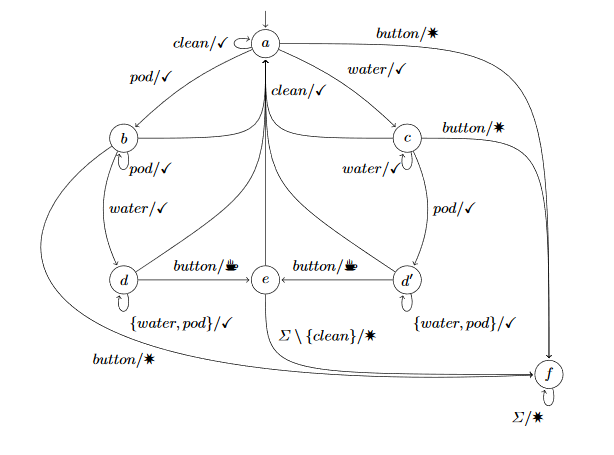
\includegraphics[width=0.7\linewidth]{content/coffeemealy}
	\caption{Mealy machine representing the functionality of a coffee machine.\cite{Steffen2011}}
	\label{fig:coffeemealy}
\end{figure}

Since automatons deal with alphabets, formal language theory is essential not only to work with them, but to build them efficiently. Often automata are used to model and test real-life systems. Naturally, questions of efficiency, correctness arise, which is why we will next expand on the relations of automatons and formal languages.

\begin{definition}[Recognized language of automata]
	The language $L\subseteq\Sigma$ containing all the accepted words by an automaton M is called the recognized language of the automaton. It is denoted by L(M) = L.
\end{definition}

\begin{definition}[Regular language]
	A formal language L is regular, iff there exists a Deterministic Finite Automaton M, for which L(M) = L, in other words, iff there exists a DFA with the recognized language of L.
\end{definition}

We will now introduce a semantic helper $\delta^*$ for both DFAs and Mealy machines. $\delta^*$ is an extension of the $\delta$ transition function, as $\delta^*: S\times\Sigma^* \to S$ defined by $\delta^*(s,\epsilon) = s$ and $\delta^*(s, \alpha w) = \delta^*(\delta(s, \alpha), w)$, essentially giving us the state of the automaton after running an input sequence from a specified state.

\begin{definition}[Myhill-Nerode relation] 
	A DFA $M=(S,s_{0},\Sigma,\delta,F)$ induces the following equivalence relation $\equiv_M$ on $\Sigma^*$ (when L(M) = $\Sigma$):\\
	\null\qquad$x\equiv_M y \iff \delta^*(s, x) = \delta^*(s, y)$\\
	where $x, y\in\Sigma^*$. This means, that x and y are equivalent with respect to $\equiv_M$.\cite{Kozen1977}.
\end{definition}

The Myhill-Nerode relation is an equivalence relation, meaning $x\equiv_M y$ is reflexive, symmetric and transitive. Also, the following properties apply to it\cite{Kozen1977}.


\begin{itemize}
	\item Right congruence: $\forall x, y\in\Sigma^*: (x\equiv_M y \implies 		\forall a\in\Sigma: xa\equiv_Mya)$\\ also, by induction, this can be extended to:\\
	$\forall x, y\in\Sigma^*: (x\equiv_M y \implies \forall w\in\Sigma^*: xw\equiv_Myw)$. 
	\item It respects membership wrt. R:\\
	$\forall x, y\in\Sigma^*: x\equiv_M y \implies (x\in R \iff y\in R)$
	\item $\equiv_M$ is of finite index, has finitely many equivalency classes. Since for every state $s\in S$, the sequences which end up in s are in the same equivalence class, the number of these classes is exactly $|S|$, which is a finite set.
\end{itemize}

Using this relation, we can introduce the Myhill-Nerode theorem, which neatly ties together the previous definitions.

\begin{theorem}[Myhill-Nerode theorem\cite{Kozen1977}\cite{10.2307/2033204}]
	Let $L\subseteq\Sigma^*$. The following three statements are equivalent:
	\begin{itemize}
		\item L is regular.
		\item there exists a Myhill-Nerode relation for L.
		\item the relation $\equiv_L$ is of finite index.
	\end{itemize}
	For proof, see \cite{Kozen1977}\cite{10.2307/2033204}.
\end{theorem}

Next, we will introduce the same topics to Mealy machines, which are a bit more complex in this regard. In order to do this, we need to introduce a semantic helper similar to $\delta^*$, but considering the output function of Mealy machines. $\lambda^*: S\times\Sigma^* \to \Omega$, defined by $\lambda^*(s, \epsilon) = \varnothing$ and $\lambda^*(s, w\alpha) = \lambda(\delta^*(s, w), \alpha)$.



When monitoring the behavior of Mealy machines, one of the most important metrics given an input is not whether it is accepted or rejected (as it would be with a DFA), but rather what specific output was caused by an input. The behavior of a Mealy machine, a specific run of it, has a pattern of \textit{$i_1,o_1,i_2,o_2,..,i_n,o_n$}, where \textit{i} are inputs and \textit{o} are outputs. But in order to characterize these runs, we actually do not need every output from this pattern, we only need the final one. This means, that a $\llbracket M\rrbracket$: $\Sigma^*\to\Omega$ semantic functional fully captures the behavioral semantics of Mealy machines. We define $\llbracket M\rrbracket$: $\Sigma^*\to\Omega$ as  $\llbracket M\rrbracket$(w) = $\lambda^*(s_0, w)$. Informally,the  $\llbracket M\rrbracket$ functional accepts a set of inputs, and returns the last output given after running them from the initial state of the automaton. 

\begin{example}
	Given the Mealy machine $M\textsubscript{coffeemachine}$ in Fig. \ref{fig:coffeemealy}, the runs:\\
	\null\qquad<clean, $\checkmark$>, \\
	\null\qquad<pod water button, \Coffeecup> \\
	are in $\llbracket M\textsubscript{coffeemachine}\rrbracket$, since these input words cause these outputs, while the runs\\
	\null\qquad<clean, \Coffeecup> and \\
	\null\qquad<water button button, $\checkmark$> \\
	are not, since these input sequences do not produce those outputs.
\end{example}

Similarly to the Myhill-Nerod relations in DFAs, we can introduce an equivalence relation over the $P: \Sigma^*\to\Omega$ functional. P being an abstraction of $\llbracket M\rrbracket$, since the latter only maps from initial states.

\begin{definition}[Equivalence of words wrt. $\equiv_P$\cite{Steffen2011}]
	Given a Mealy machine $M=(S,s_{0},\Sigma,\Omega,\delta,\lambda) $, two words, $u, u'\in\Sigma^*$ are equivalent with respect to $\equiv_P$:\\
	$u \equiv_P u' \iff (\forall v\in\Sigma^*:P(s, uv) = P(s, u'v))$.\\
	We write [u] to denote the equivalence class of u wrt. $\equiv_P$.
\end{definition}

This definition is more along the lines of the right congruence property observed in the Myhill-Nerode relations, the original ($u \equiv_P u' \iff P(s, u) = P(s, u')$) format would of course still hold, in this case, $v = \epsilon$.

\begin{example}
	Taking Fig. \ref{fig:coffeemealy} as an example, the following words are equivalent wrt. $\equiv_{\llbracket M\rrbracket}$:\\
	\null\qquad\qquad\qquad\qquad\space water, pod\\
	\null\qquad\qquad$\equiv_{\llbracket M\rrbracket}$\qquad water, water, pod\\
	\null\qquad\qquad$\equiv_{\llbracket M\rrbracket}$\qquad pod pod water.
	
	The first two of these are straightforward, since both lead to the same state, $d'$, more interesting is the \textit{pod pod water} input, which ends in state $d$. Observably, state $d$ and $d'$ wrt. outputs operate exactly the same regardless of continuation, this is why the equivalence holds.
\end{example}

\begin{theorem}[Characterization theorem\cite{Steffen2011}]
	Iff mapping $P: \Sigma^*\to\Omega$ $\equiv_P$ has finitely many equivalence classes, there exists a Mealy machine M, for which P is a semantic functional.
	\\\\
	\textit{Proof}($\impliedby$): As seen in the case of the Myhill-Nerode finite index property for DFAs, same states in Mealy machines will obviously be in same equivalence classes. This implies, that the number of classes in (or in other words, the index of) $\equiv_P$ is at most the number of states the Mealy machine contains, which is finite by definition.
	\\
	\textit{Proof}($\implies$): Consider the following Mealy machine: $M_P=(S,s_{0},\Sigma,\Omega,\delta,\lambda)$:\\
	\null\qquad -S is given by the equivalence classes of $\equiv_P$.\\
	\null\qquad -$s_0$ is given by $[\epsilon]$.\\
	\null\qquad -$\delta$ is defined by $\delta([u], \alpha) = [u\alpha]$.\\
	\null\qquad -$\lambda$ is defined by $\lambda([u], \alpha) = o$, where $P(u\alpha) = o$.\\
	A Mealy machine constructed this way fulfills what the theorem states, P is a semantic functional of it, in other words, $\llbracket M\rrbracket$ = P.
\end{theorem}

With this theorem, we can define regularity for mappings $P:\Sigma^*\to\Omega$. We call a $P:\Sigma^*\to\Omega$ mapping regular, iff there exists a corresponding Mealy machine for which $\llbracket M\rrbracket$ = P, or equivalently, if P has a finite number of equivalence classes, analogously to the previously seen "classical" regularity.

The introduction of regularity helps us in the construction of automata, specifically, the construction of canonical automata. 

\begin{definition}[Minimal automata]
	An automata M recognizing the language L is minimal iff every $M'\neq M$ automata that also recognize L have at least as many states as M.
\end{definition}

\begin{figure}[H]
	\centering
	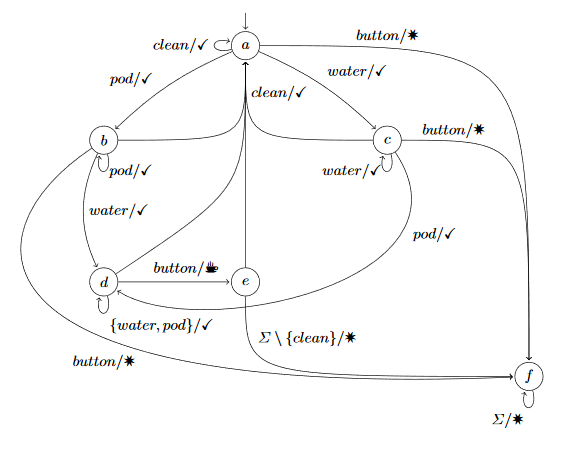
\includegraphics[width=0.7\linewidth]{include/coffeemealyminimal}
	\caption{Minimal version of the Mealy machine seen in \ref{fig:coffeemealy}}
	\label{fig:coffeemealyminimal}
\end{figure}


\begin{definition}[Canonical automaton]
	An automaton accepting the language L is canonical iff it is minimal, and contains every other automaton that accepts L.
\end{definition}


Constructing automata to be canonical, especially in the case of Mealy machines is important with regards to efficiency and is the backbone of automaton learning. We will steer to algorithm theory that does this, before actually covering the topic of automaton learning itself. The next proposition comes straightforward from the previously presented characterization theory.


\noindent \textbf{Proposition (Bounded reachability\cite{Steffen2011})}: Every state of a minimal Mealy machine with n states has an access sequence, i.e., a path from the initial state to this  state,  of  length  at  most n−1.  Every  transition  of  this  Mealy  machine  can be covered by a sequence of length at most n from the initial state.

The process of constructing automata will use the concept of partition refinement. It works based on distinguishing suffixes, suffixes of words which mark, witness the difference between two access sequences. We'll introduce the following notion to formalize this.


\begin{definition}[k-distinguishability\cite{Steffen2011}]
	Two states, $s,s'\in S$ are k-distinguishable iff there is a word $w\in\Sigma^*$ of length k or shorter, for which $\lambda^*(s, w)\neq\lambda^*(s',w)$.
\end{definition} 

\begin{definition}[exact k-distinguishability]
	Two states, $s,s'\in S$ are exact k-distinguishable, denoted by $k^=$ iff s and s' are k-distinguishable. but not (k-1)-distinguishable
\end{definition}

Essentially, if two states, s and s' are  k-distinguishable, then when processing the same input sequence, from some suffix of the word w with length at most k, they will produce differing outputs. Using this, we can observe, that whenever two states, $s_1, s_2\in S$ are (k+1)-distinguishable, then they each have an $\alpha$-successor, $s_1'$ and $s_2'$ for some $\alpha\in\Sigma$, such that $s_1'$ and $s_2'$ are k-distinguishable. This suggests, that:
\begin{itemize}
	\item no states are 0-distinguishable and
	\item two states $s_1$ and s2 are (k+1)-distinguishable iff there exists an input symbol $\alpha\in\Sigma$, such that $\lambda(s_1, \alpha) \neq \lambda(s_2,\alpha)$ or $\delta(s_1, \alpha)$ and $\delta(s_2, \alpha)$ are k-distinguishable.
\end{itemize}
This way, if we have an automaton M, we can construct its minimal version, by iteratively computing k-distinguishability for increasing k until stability, that is until the set of exactly k-distinguishable states is empty.

\begin{example}
	Given the Mealy machine seen in Fig.\ref{fig:coffeemealy}, we can use k-distinguishability to refine its partitions. The initial state, the initial partition would be:\\
	$P_1 = \{a, b, c\}, \{d, d'\}, \{e\}, \{f\}$\\
	since when k=1, a, b and c are not 1-distinguishable, but d and d' separate on the behavior of the \textit{button} input, while e and f are separated by the suffix \textit{clean}. Let's see the k=2 scenario.\\
	$P_2 = \{a\}, \{b\}, \{c\}, \{d, d'\}, \{e\}, \{f\}$\\
	Here, \textit{water} and \textit{pod} separate a, b and c, while d and d' can still no longer be separated. If observed, even if k is increased, d and d' can not be refined. This means, that they are indistinguishable, they can be merged together without altering behavior. This shows the process of acquiring the minimal machine seen in Fig. \ref{fig:coffeemealyminimal}.
	\label{ex:partitionrefinement}
\end{example} 

The process explained in the above example is partition refinement, the exact algorithm and proof of its validity can be seen in \cite{Steffen2011}, it is a version of the minimization algorithm for DFAs proposed by Hopcroft\cite{HOPCROFT1971189}. 

We will define one last relation which will help us in the next section to compare automata minimization and automata learning.

Let  $M=(S,s_{0},\Sigma,\Omega,\delta,\lambda)$ and $M=(S',s_{0}',\Sigma,\Omega,\delta',\lambda')$ be two Mealy machines with shared alphabets. We call a surjective function $f_k: S \to S'$ existential k-epimorphism between $M$ and $M'$, if for all $s'\in S', s\in S$ where $f_k(s) = s'$ and with any $\alpha\in\Sigma$, we have: $f_k(\delta(s,\alpha)) = \delta'(s',\alpha)$, and all states, that are mapped by $f_k$ to the same state of $M'$ are not k-distinguishable. It is straightforward to establish that all intermediate models arising during the partition refinement process are images of the considered Mealy machine under a k-epimorphism, where k is the number of times all transitions have been investigated.\cite{Steffen2011} Essentially this establishes $P_1$ and $P_2$ from Example \ref*{ex:partitionrefinement} as images of the Mealy machine seen in Fig. \ref{ex:coffeemealy} under k-epimorphisms where k=1 and k=2 respectively.

Active automaton learning algorithms operate in a very similar way, but they are not the same as minimization algorithms, since they do not have access to the automatons they are learning. We will extend upon this in the next section.



\section{Automaton learning}



\paragraph{Automaton learning}  is modeling a system without having specific knowledge of its the internal behavior. To accomplish this, a model needs to be inferred by observing the external behavior of the system. This learned model is, as the name suggests, an automaton. 
\\Formally: Active  automata  learning is  concerned  with  the  problem  of  inferring  an automaton model for an unknown formal language $L$ over some alphabet $\Sigma$\cite{Howar2018}.
\\\\In order to monitor a system, a way of access to its behavioral information is required. There are two approaches, which separate the two types of automaton learning as well.

\paragraph{Passive automaton learning} In case of passive automaton learning, the gathering of information is not part of the learning process, but rather a prerequisite to it. The learning is performed on a pre-gathered positive an/or negative example set of the systems behavior. In passive automaton learning, the success of the process is determined not only by the efficiency of the algorithm, but the methodology and time used to gather the data.

\paragraph{Active automaton learning} In case of active automaton learning, the behavioral infromation is gathered by the learning algorithm in an "active" way via queries. In order to accomplish this, learning is separated to two components: the learner, which learns, and the teacher, which can answer questions about the system under learning.


Active automaton learning follows the MAT, or the Minimally Adequate Teacher model proposed by Dana Angluin\cite{ANGLUIN198787}. It separates the algorithm to a learner and a teacher, where the teacher can only answer the minimally adequate questions needed to learn the system. These two questions, or queries are are follows:


\paragraph{Membership query} Given a $w\in\Sigma^{*}$ word, the query return the $o\in \Omega$ output corresponding to it, treating the word as a string of inputs. We write $mq(w) = o$ to denote that executing the query w on the system under learning (SUL) leads to the output o: $\llbracket SUL \rrbracket(w) = o$ or $\lambda^*(s_0, w) = o$.

\paragraph{Equivalence query} Given a hypothesis automaton $M$, the query tries to determine if the hypothesis is behaviorally equivalent to the SUL, and if not, finding the diverging behavior, and return with the example of it. We write $eq(H) = c$, where $c\in\Sigma^*$, to denote an equivalence query on hypothesis H, returning a counterexample c. The counter example provided is the sequence of inputs for which the output of system under learning and the output of the hypothesis differ: $ \llbracket H\rrbracket(c) \neq mq(c)$.

\noindent The learner component uses membership queries to construct a hypothesis automaton, then refines this hypothesis by the counterexamples provided by equivalence queries. Once counterexamples can not be found this way, the learners hypothesis is behaviorally equivalent to the SUL, the learning can terminate and the output of the learning is the current hypothesis.

\begin{figure}[H]
	\centering
	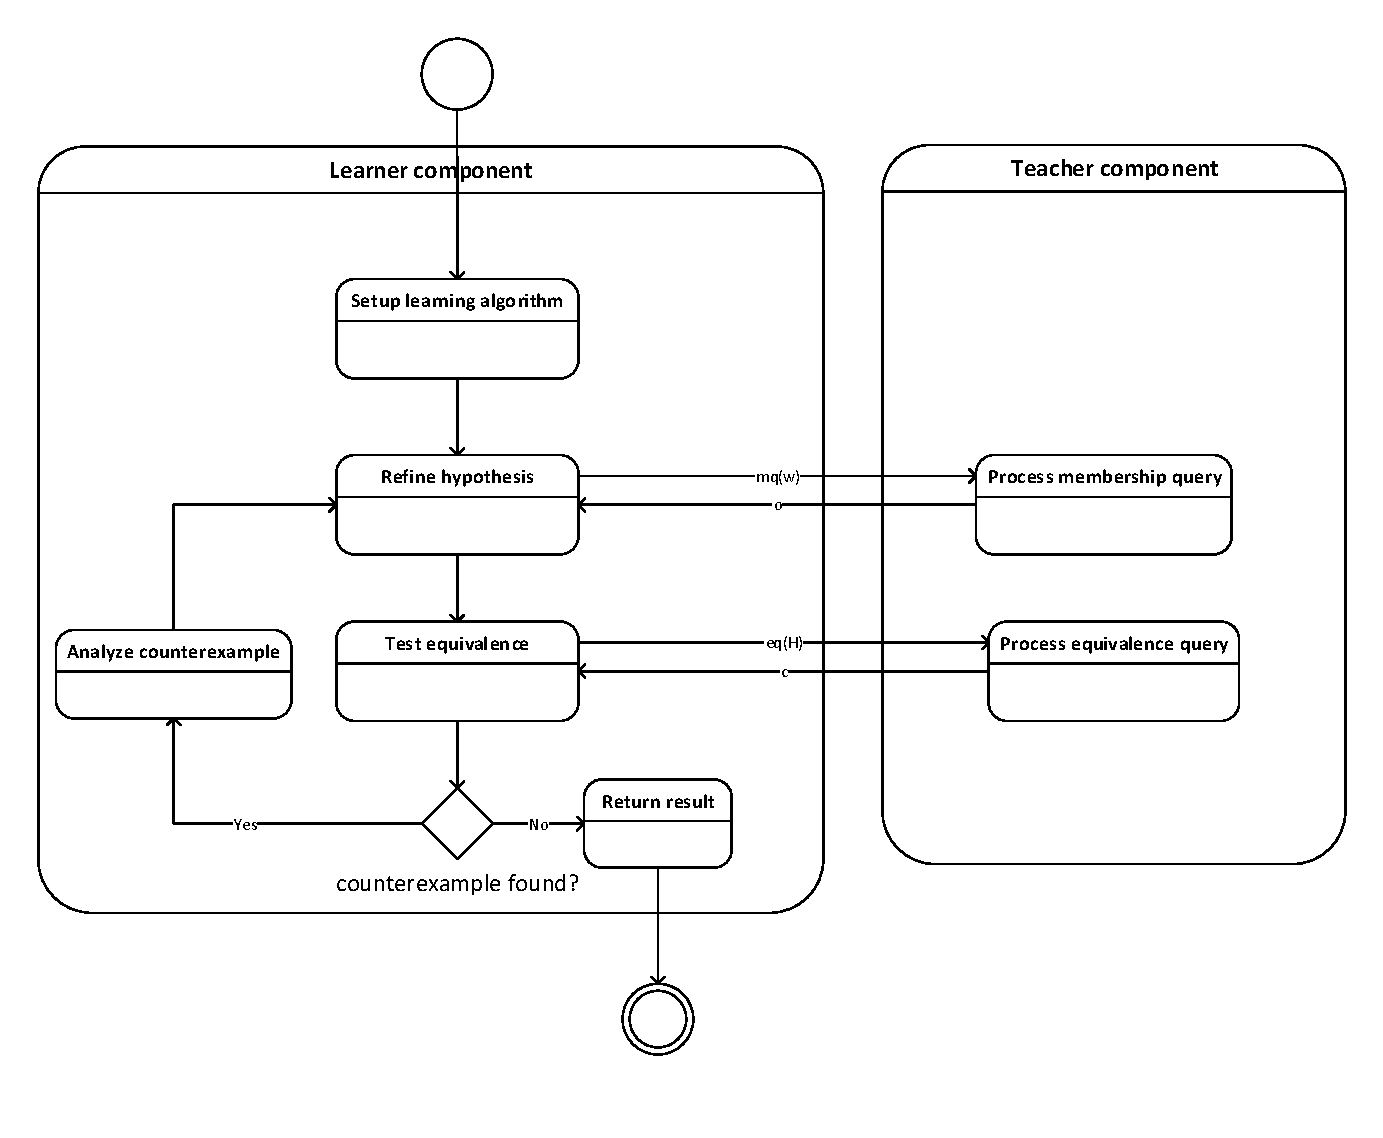
\includegraphics[width=1.0\linewidth]{figures/flowchartlearning}
	\caption{Abstract model of active automata learning algorithms}
	\label{fig:flowchartlearning}
\end{figure}

As seen on Fig. \ref{fig:flowchartlearning}, the learning proceeds in rounds, generating and refining hypothesis models by exploring the SUL via membership queries. As the equivalence checks produce counterexamples, the next round of this hypothesis refinement is steered by the counterexamples produced.

Using an analogous strategy to the minimization of automatons seen in the previous section, starting only with a one state hypothesis automaton, we explore over all words in the alphabet in order to refine and extend it. Here, there is a dual way of characterizing (and distinguishing) between states\cite{Steffen2011}:
\begin{itemize}
	\item By words reaching them. A prefix-closed set of $S_p$ words, reaching each state exactly once, defines a spanning tree of the automaton. This characterization aims at providing exactly one representative element from each class of $\equiv_P$ on the SUL. Active learning algorithms incrementally construct such a set $S_p$. \\This prefix-closedness is necessary for $S_p$ to be a "spanning tree" of the Mealy machine. Extending $S_p$ with all the one-letter continuations of words in $S_p$ will result in the tree covering all the transitions of the Mealy machine. $L_p$ will denote all the one-letter continuations that are not already contained in $S_p$.
	\item By their future behavior with respect to an increasing vector of words of $\Sigma^*$. This vector $<d_1, d_2,...,d_k>$ will be denoted by $D$, and contains the "distinguishing suffixes". The corresponding future behavior of a state, here given in terms of its access sequence $u\in S_p$, is the output vector$<mq(u*d_1), ..., mq(u*d_k)>\in\Omega^k$, which leads to an upper approximation of the classes of $\equiv_{\llbracket SUL\rrbracket}$. Active learning incrementally refines this approximation by extending the vector until the approximation is precise.
\end{itemize}
While the second characterization defines the states of the automaton, where each output vector corresponds to one state, the spanning tree on $L_p$ is used to determine the transitions of these states. In order to characterize the relation between the SUL $M=(S,s_{0},\Sigma,\Omega,\delta,\lambda)$ and the hypothesis model $M'=(S',s_{0}',\Sigma,\Omega,\delta',\lambda')$ (note, that $M$ and $M'$ only share alphabets) let $D\subseteq\Sigma^*$. We call a surjective function $f_D:S\to S'$ existential D-epimorphism (surjective homomorphism) between $M$ and $M'$ if, for all $s'\in S'$ there exists an $s\in S$ with $f_D(s) = s'$ such that for all $\alpha \in \Sigma$ and all $d\in D$: $f_D(\delta(s, \alpha)) = \delta'(s', \alpha)$, and $\lambda^*(s,d) = \lambda^*(s', d)$. \\
Note, that active learning deals with canonical Mealy machines, in other words, the canonical form of SUL, and not, the perhaps much larger Mealy machine of SUL itself. \\

Since active learning algorithms maintain an incrementally growing extended spanning tree for $H=(S_H, h_0, \Sigma, \Omega, \delta_H, \lambda_H)$, i.e., a prefix-closed set of words reaching all its states and covering all transitions, it is straightforward to establish that these hypothesis models are images of the canonical version of SUL under a canonical existential D-epimorphism, where D is the set of distinctive futures underlying the hypothesis construction\cite{Steffen2011}
\begin{itemize}
	\item define $f_D : S_{SUL}\to S_H$ by $f_D(s) = h$ as following: if $\exists w\in S_p \cup L_p$, where $\delta(s_0, w) = s$, then $h = \delta_H(h_0,w)$. Otherwise h may be chosen arbitrarily.
	\item It suffices to consider the states reached by words in the spanning tree to establish the defining properties of $f_D$. This straightforwardly yields:
	\begin{itemize}
		\item $f_D(\delta(s,\alpha)) = \delta_H(h, \alpha)$ for all $\alpha\in\Sigma$, which reflects the characterization from below.
		\item $\lambda^*(s, d) = \lambda^*_H(h,d)$ for all $d\in D$, which follows from the maintained characterization from above.\cite{Steffen2011}
	\end{itemize}
\end{itemize}

In basic logic, D-epimorphisms and k-epimorphisms do not differ, they both deal with establishing constructed models being images of the model they are based on. D-epimorphisms could replace k-epimorphisms where $D=\Sigma^k$, it can be suggested, that there is no need to differentiate. However, the there is in important difference of complexity between the two. While k-distinguishability supports polynomial time, black-box systems do not. Also, the "existential" in existential D-epimorphism is important: $f_D$ must deal with unknown states, ones that haven't been encountered yet. This implies that characterization can only be valid for already encountered states.

Active learning algorithms can be proven correct using the following three-step pattern:
\begin{itemize}
	\item Invariance: The number of states of each hypothesis has an upper bound of $\equiv_{\llbracket SUL\rrbracket}$.
	\item Progress: Before the final partition is reached, an equivalence query will provide a counterexample, where an input word leads to a different output on the SUL and on the hypothesis. This difference can only be resolved by splitting at least one state, which increases the state count.
	\item Termination: The refinement terminates after at most the index of $\equiv_{\llbracket SUL\rrbracket}$ many steps, caused directly by the described invariance and progress properties.
\end{itemize}

The following subsection introduces the first active automaton learning algorithm this thesis covers.

\subsection{Direct Hypothesis Construction}
The Direct Hypothesis Construction algorithm, as seen in Algorithm \ref{algo:dhc}  follows the idea of the breath-first search of graph theory, it constructs the hypothesis using a queue of states, which is initialized with the states of the spanning tree to be maintained. Explored states are removed from this queue, while the discovered successors are enqueued, if they are provably new states. The algorithm starts with a one-state hypothesis, including only the initial state, reached by $\epsilon$ and D = $\Sigma$. It then tries to complete the hypothesis, for every state we determine the behavior of the state under D, which we will call the extended signature of said state. States with a new extended signatures are provably new states, so to guarantee further investigation, we enqueue all their successors. Initially, $D=\Sigma$, so only the $1^=$-distinguishable states are revealed during the first iteration. This is extended straightforwardly to comprise a prefix closed set of access sequences.\cite{Steffen2011}\cite{10.1007/978-3-642-34781-8_19}

\begin{algorithm}[H]
	\KwIn{$S_p$: a set of access sequences, D: a set of suffixes, an input alphabet $\Sigma$}
	\KwOut{A Mealy machine $H=(S, s_0, \Sigma, \Omega, \delta, \lambda)$}
	initialize hypothesis H, create a state for all elements of $S_p$\;
	initialize a queue Q with the states of H\;
	\While{Q is not empty}{
		s = dequeue state from Q\;
		u = access sequence from $s_0$ to s\;
		\For{$d\in D$}{
			o = mq($u\*d$)\;
			set $\lambda(s,d) = o$\;
		}
		\eIf{exists an $s'\in S$, where the output signature of $s'$ is the same as $s$}{
			reroute transitions of $s$ to $s'$ in H\;
			remove $s$ from H\;
		}{
			create and enqueue successors of $s$ for every input in $\Sigma$ into Q\;
		}
	}
	\caption{The Direct Hypothesis Construction algorithm as seen in \cite{Steffen2011}.}
	\label{algo:dhc}
\end{algorithm}

